\section{Model-Free Reinforcement Learning}
\label{sec:mf_rl}

Model based methods are based on solving Bellman equation \eqref{eqn:bellman_v}, \eqref{eqn:bellman_q} with a given model $T$. 
On the other hand, Model-Free Reinforcement Learning is suitable 
if environment model is not available but the agent can experience environment by the consequences of its actions. There are three main categories in model-free RL:  

\begin{description}
	\item[Value-Based Learning] The value functions are learned, 
	hence the policy arises naturally from the value function using  \eqref{eqn:policy_stochastic_q} and \eqref{eqn:policy_deterministic_q}. 
	Since $\argmax$ operation is used, this type of learning is suitable for problems where action space is discrete. 
	
	\item[Policy-Based Learning] The policy is learned directly, 
	and return values are used instead of learning a value function. 
	Unlike value-based methods, it is suitable when continuous action spaces are available in the environment. 
	
	\item[Actor-Critic Learning] Both policy (actor) and value (critic) functions are learned simulatenously. 
	Thus, it is also suitable for continuous action spaces. 
	
\end{description}

\subsection{Q Learning}
Q Learning is a value-based type of learning. 
It is based on optimizing $Q$ function using Bellman Equation \eqref{eqn:bellman_q}~\cite{watkins_technical_1992}. 
In this learning strategy, $Q$ function is assumed to be parametrized by $\theta$. 
Target $Q$ value is estimated by bootstrapping estimate, 
\begin{equation}
\label{eqn:q_target}
Y_t^Q = r_t + \gamma \max_{a'} Q(s_{t+1},a';\theta).
\end{equation}
At time $t$,  with state, action, reward, next state tuples ($s_t,a_t,r_t,s_{t+1}$), 
$Q$ values are updated by minimizing difference between the target value and the estimated value.
Hence the loss 
\begin{equation}
\label{eqn:q_loss}
\mathcal{L}_t(\theta) = \big( Y_t - Q(s_t,a_t;\theta) \big) ^ 2, 
\end{equation}
is to be minimized with respect to $\theta$ using numerical optimization methods. 

\subsubsection{Deep Q Learning}
When a nonlinear approximator is used for $Q$ estimation, learning is unstable due to the correlation among recent observations, hence correlations between updated $Q$ function and observations.
Deep Q Learning solves this problem by introducing Target Network and Experience Replay \cite{mnih_human-level_2015, mnih_playing_2013} along with using deep neural networks. 

\textbf{Target Network} is parametrized by $\theta^-$. 
It is used to evaluate target value, but it is not updated by the loss minimization. 
It is updated at each fixed number of update step by Q network parameter $\theta$. 
In this way, correlation between target value and observations are reduced.
The target value is obtained by using $\theta^-$ as
\begin{equation}
\label{eqn:dqn_ntarget}
Y_t^{DQN} = r_t + \gamma \max_{a'} Q(s_{t+1},a';\theta^-).
\end{equation}

\textbf{Experience Replay} stores experience tuples in the replay memory $\mathcal{D}$ as a queue with fixed buffer size $N_{replay}$. 
At each iteration $i$, $\theta$ is updated by experiences $(s,a,r,s')\sim U(\mathcal{D})$ uniformly subsampled from experience replay by minimizing the expected loss
\begin{equation}
\label{eqn:dqn_loss}
\mathcal{L}_i(\theta_i) = \mathbb{E}_{(s,a,r,s')\sim U(\mathcal{D})}\Big[\big( Y^{DQN} - Q(s,a;\theta_i) \big) ^ 2 \Big].
\end{equation}
It allows agent to learn from experiences multiple times at different stages of learning. 
More importantly, sampled experiences are close to be independent and identically distributed if buffer size is large enough. 
Again, this reduces correlation between recent observations and updated $Q$ value. This makes learning process more stable. 

\textbf{Epsilon Greedy Exploration} is used to let agent explore environment. 
In discrete action space (finite action space $\mathcal{A}$), this is 
the simplest exploration strategy used in RL algorithms.
During the learning process, a random action with probability $\epsilon$ is selected or greedy action (maximizing Q value) with probability $1-\epsilon$. In order to construct policy:   
\begin{equation}
\label{eqn:egreedy_policy}
\pi(a|s) = 
\begin{cases}
1-\epsilon,   & \text{if } a = \argmax_{a} Q(s, a), \\
\frac{\epsilon}{|\mathcal{A}|-1},     & \text{otherwise}.
\end{cases}
\end{equation}
where $|\mathcal{A}|$ denotes cardinality of $\mathcal{A}$. 
In Algorithm~\ref{alg:dqn}, we summarize the Deep Q Learning with Experience Replay. 

\begin{algorithm}[H]
	\SetAlgoLined
	\DontPrintSemicolon % Some LaTeX compilers require you to use \dontprintsemicolon instead
	Initialize: $\mathcal{D}$, $N$, $N_{replay}$, $\theta$, $\epsilon$, $d$ \\
	$\theta^- \leftarrow \theta$ \\
	\For{$\text{episode} = 1, M $}{
		Recieve initial state $s_1$; \\
		\For{$t = 1, T$}{
			Randomly select action $a_t$ with probability $\epsilon$, otherwise $a_t = \arg\max_{a} Q(s_t, a; \theta)$ greedily; \\
			Execute action $a_t$ and recieve reward $r_t$ and next state $s_{t+1}$; \\
			Store experience tuple $e_t = (s_t, a_t, r_t, s_{t+1})$ to $\mathcal{D}$ ; \\
			Sample random batch $\mathcal{D}_{r}$ ($|\mathcal{D}_{r}|=N$) from $\mathcal{D}$; \\
			$Y_j = \begin{cases}
			r_j & \text{if } s_{j+1} \text{ terminal, } \\
			r_j + \gamma \max_{a'} Q(s_{j+1},a';\theta^-) & \text{otherwise, } 
			\end{cases}$, $\forall e_j \in \mathcal{D}_{r}$\\
			Update $\theta$ by minimizing $ \frac{1}{N}\sum_{e_j \in \mathcal{D}_{r}} \big[ Y_j - Q(s_j,a_j;\theta) \big] ^ 2$ for a single step; \\
			\lIf{$t \mod d$}{
				Update target network: $\theta^- \leftarrow \theta$;
			}
		}
	}
	\caption{Deep Q Learning with Experience Replay}
	\label{alg:dqn}
\end{algorithm}

\subsubsection{Double Deep Q Learning}
In DQN, maximum operator is used to both select and evaluate action on the same network as in \eqref{eqn:dqn_ntarget}. 
This yields overestimation of $Q$ function in noisy environments. 
Therefore, action selection and value estimation is decoupled in target evaluation to overcome $Q$ function overestimation~\cite{van_hasselt_deep_2015} using Double Deep Q Network (DDQN). 
The target value in this approach can therefore be written as follows:
\begin{equation}
\label{eqn:ddqn_ntarget}
Y_t^{DDQN} = r_t + \gamma Q(s_{t+1}, \arg\max_{a'} Q(s_{t+1}, a'; \theta_i );\theta^-).
\end{equation}
Except the target value, the learning process is the same as in DQN. 

\subsection{Actor-Critic Learning}

Value-based methods are not suitable for continuous action spaces. 
Therefore, policy should be explicitly defined instead of maximizing $Q$ function. 
For such problems, actor-critic type learning methods use both value and policy models seperately. 

In actor-critic learning, there exists two components~\cite{silver_deterministic_2014}:  
First one is the actor, which is the policy function, either stochastic or deterministic, parametrized by $\theta^{\pi}$ or $\theta^{\mu}$, respectively. 
For policy learning, an estimate of the value function is used instead of the true value function since it is already unknown. 
Second one is the critic, which is an estimator of the $Q$ value, parametrized by $\theta^Q$. 
Critic learning is achieved by minimizing the error obtained by either Monte Carlo sampling or Temporal Difference bootstrapping.
Critic is what policy uses for value estimation. 

The ultimate goal is to learn a policy maximizing the value function $V$ by selecting action which maximizes $Q$ value in \eqref{eqn:policy_deterministic_q}. 
Therefore, value function is the criteria to be maximized by solving parameters $\theta^\pi$ (or $\theta^\mu$) given $\theta^Q$. 
At time $t$, the loss function for the policy is negative, that is,  
\begin{equation}
\label{eqn:ac_value_maximization}
\mathcal{L}_t(\theta^\pi) = - Q(s_t, \widetilde{a}_t;\theta^Q), \quad \widetilde{a}_t \sim \pi(\cdot|s_t;\theta^\pi).
\end{equation}

In order to learn policy $\pi$, $Q$ function should also be learned simultaneously. 
For $Q$ function approximation, the target value is parametrized by $\theta^Q$ and $\theta^\pi$,
\begin{equation}
\label{eqn:ac_target}
Y_t^{AC} = r_t + \gamma Q(s_{t+1}, \widetilde{a}_{t+1});\theta^Q), \quad \widetilde{a}_{t+1} \sim \pi(\cdot|s_{t+1};\theta^{\pi}),
\end{equation}
and this target is used to learn $Q$ function by minimizing the least squares loss (in general),
\begin{equation}
\label{eqn:ac_loss}
\mathcal{L}_t(\theta^Q) = \big[ Y_t^{AC} - Q(s_t,a_t;\theta^Q) \big] ^ 2.
\end{equation}

Note that both the actor and the critic should be learned at the same time. Therefore, parameters are updated simultaneously during the iterations in the learning process. 

\subsubsection{Deep Deterministic Policy Gradient}
DDPG is continuous complement of DQN using a deterministic policy~\cite{lillicrap_continuous_2019}. 
It also uses experience replay and target networks. 
Similar to Deep Q Learning, there are target networks parametrized by $\theta^{\mu^-}$ and $\theta^{Q^-}$ 
along with the main networks parametrized by $\theta^{\mu}$ and $\theta^{Q}$. 

While target networks are updated in a fixed number of steps in DQN, 
DDPG updates target network parameters at each step with Polyak averaging, 
\begin{equation}
\label{eqn:target_update}
\theta^- \leftarrow \tau \theta + (1-\tau) \theta^- .
\end{equation}
The $\tau$ is an hyperparameter indicating how slow the target network is updated and it is usually close to zero. 

Policy network parameters are learned by maximizing resulting expected value, or minimizing its negative,
\begin{equation}
\label{eqn:ddpg_policy_loss}
\mathcal{L}_i(\theta^\mu_i) = -\mathbb{E}_{s \sim U(\mathcal{D})} \Big[ Q(s, \mu(s\theta^\mu_i);\theta^Q) \Big].
\end{equation} 
Note that value network parameters are also assumed to be learned. 

In addition, target networks are used to predict target value and the target is defined by
\begin{equation}
\label{eqn:ddpg_target}
Y_t^{DDPG} = r_t + \gamma Q(s_{t+1}, \mu(s_{t+1};\theta^{\mu^-});\theta^{Q^-}).
\end{equation}
In each iteration, this target is used to learn $Q$ function by minimizing the least squares loss 
\begin{equation}
\label{eqn:ddpg_loss}
\mathcal{L}_i(\theta^Q_i) = \mathbb{E}_{s,a,r,s'\sim U(\mathcal{D})}\Big[\big( Y^{DDPG} - Q(s,a;\theta^Q_i) \big) ^ 2 \Big].
\end{equation}

In DDPG, value and policy network parameters are learned simultaneously. 
During the learning process, exploration noise is added to each selected action. 
In ~\cite{lillicrap_continuous_2019}, authors proposed to use Ornstein-Uhlenbeck Noise~\cite{uhlenbeck_theory_1930} in order to have temporal correlation for efficiency. 
However, a simple Gaussian white noise or any other one is also possible. 

DDPG is summarized in Algorithm \ref{alg:ddpg}. 

\begin{algorithm}[H]
	\SetAlgoLined
	\DontPrintSemicolon % Some LaTeX compilers require you to use \dontprintsemicolon instead
	Initialize: $\mathcal{D}$, $N$, $N_{replay}$, $\theta^{\mu}$, $\theta^Q$, $\mathcal{X}$ \\
	$\theta^{\mu^-} \leftarrow \theta^{\mu}$, $\theta^{Q^-} \leftarrow \theta^{Q}$ \\
	\For{$\text{episode} = 1, M $}{
		Recieve initial state $s_1$; \\
		\For{$t = 1, T$}{
			Select action $a_t = \mu(s_t; \theta^{\mu}) + \epsilon$ where $\epsilon \sim \mathcal{X}$; \\
			Execute action $a_t$ and recieve reward $r_t$ and next state $s_{t+1}$; \\
			Store experience tuple $e_t = (s_t, a_t, r_t, s_{t+1})$ to $\mathcal{D}$ ; \\
			Sample random batch $\mathcal{D}_{r}$ ($|\mathcal{D}_{r}|=N$) from $\mathcal{D}$; \\
			$Y_j = \begin{cases}
			r_j & \text{if } s_{j+1} \text{ terminal, } \\
			r_j + \gamma Q(s_{j+1},\mu(s_{j+1}; \theta^{\mu^-}); \theta^{Q^-}) & \text{otherwise, }
			\end{cases}$, $\forall e_j \in \mathcal{D}_{r}$ \\
			Update $\theta^Q$ by minimizing $ \frac{1}{N}\sum_{e_j \in \mathcal{D}_{r}} \big( Y_j - Q(s_j,a_j;\theta^Q) \big) ^ 2$ for a single step; \\
			Update $\theta^{\mu}$ by maximizing $ \frac{1}{N}\sum_{e_j \in \mathcal{D}_{r}} Q(s_j,a_j;\theta^Q)$ for a single step; \\
			Update target networks: \\
			$\theta^{\mu^-} \leftarrow \tau \theta^{\mu} + (1-\tau) \theta^{\mu^-}$ and \\
			$\theta^{Q^-} \leftarrow \tau \theta^{Q} + (1-\tau) \theta^{Q^-}$;
		}
	}
	\caption{Deep Deterministic Policy Gradient}
	\label{alg:ddpg}
\end{algorithm}

\textbf{Ornstein-Uhlenbeck Process} is the continuous analogue of the discrete first order autoregressive (AR(1)) process~\cite{uhlenbeck_theory_1930}. 
The process $x$ is defined by a stochastic differential equation,
\begin{equation}
\label{eqn:ou_process}
\frac{dx}{dt} = -\theta x + \sigma \eta(t),
\end{equation}
where $\eta(t)$ is a white noise. 
Its standard deviation in time is equal to $\frac{\sigma}{\sqrt{2\theta}}$. 
This process is commonly used as an exploration noise in physical environments since it has temporal correlation. 
Two sample paths of the process are shown in  \figref{fig:ou_vs_gaussian} in order to compare with the Gaussian noise.

\begin{figure}
	\centering
	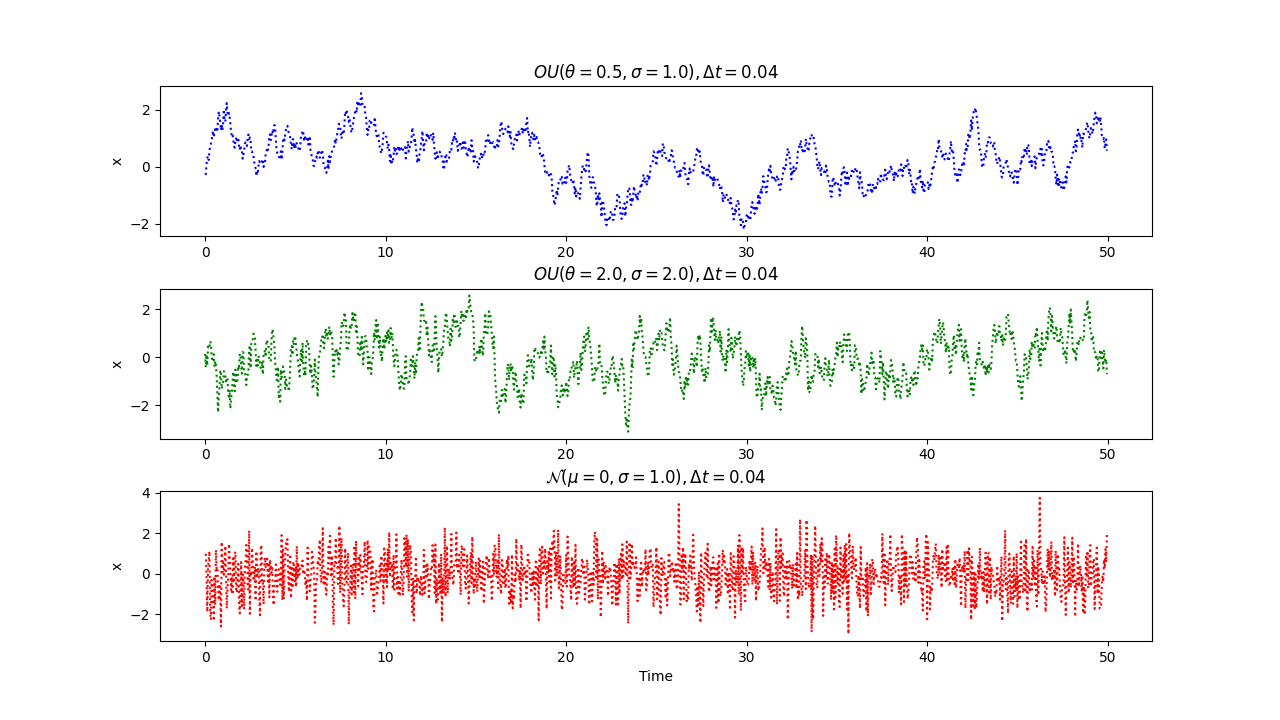
\includegraphics[width=0.98\textwidth]{figures/others/random_processes.png}
	\caption{Ornstein-Uhlenbeck Process and Gaussian Process comparison}
	\label{fig:ou_vs_gaussian}
\end{figure}

\subsubsection{Twin Delayed Deep Deterministic Policy Gradient}
TD3~\cite{fujimoto_addressing_2018} is an improved version of DDPG with higher stability and efficiency. 
There are three main tricks upon DDPG: 

\textbf{Target Policy Smoothing} is to regularize the learning process by smoothing effects of actions on value. For target value assessing, actions are obtained from the target policy network in DDPG, while a clipped zero-centered Gaussian noise is added to actions in TD3 as follows: 
\begin{equation}
\label{eqn:td3_target_action}
\widetilde{a}' = \mu(s';\theta^{\mu^-}) + \text{clip}(\epsilon, -c, c), \quad \epsilon \sim \mathcal{N}(0, \sigma).
\end{equation}

\textbf{Clipped Double Q Learning} is to escape from $Q$ value overestimation. 
There are two different value networks with their targets. 
During learning, both networks are trained by single target value assessed by using whichever of the two networks give smaller. 
In other words, 
\begin{equation}
\label{eqn:td3_target}
Y_t^{TD3} = r_t + \gamma \min_{k\in\{1,2\}} Q(s_{t+1}, ;\widetilde{a}_{j+1};\theta^{Q_k^-}).
\end{equation}
On the other hand, the policy is learned by maximizing the output of the first value network, or minimizing its negative,
\begin{equation}
\label{eqn:td3_policy_loss}
\mathcal{L}_i(\theta^\mu_i) = -\mathbb{E}_{s \sim U(\mathcal{D})} \Big[ Q(s, \mu(s;\theta^\mu_i);\theta^{Q_1}) \Big].
\end{equation} 

\textbf{Delayed Policy Updates} is used for stable training. 
During learning, policy network and target networks are updated less frequently (at each fixed number of steps) than the value network. 
Since the policy network parameters are learned by maximizing the value network, they are learned slower.  

TD3 is summarized in Algorithm \ref{alg:td3}. 

\begin{algorithm}[H]
	\SetAlgoLined
	\DontPrintSemicolon % Some LaTeX compilers require you to use \dontprintsemicolon instead
	Initialize: $\mathcal{D}$, $N$, $N_{replay}$, $\theta^{\mu}$, $\theta^Q_1$, $\theta^Q_2$, $\mathcal{X}$, $\sigma$, $c$, $d$ \\
	$\theta^{\mu^-} \leftarrow \theta^{\mu}$, $\theta^{Q^-}_1 \leftarrow \theta^{Q}_1$, $\theta^{Q^-}_2 \leftarrow \theta^{Q}_2$ \\
	\For{$\text{episode} = 1, M $}{
		Recieve initial state $s_1$; \\
		\For{$t = 1, T$}{
			Select action $a_t = \mu(s_t; \theta^{\mu}) + \epsilon$ where $\epsilon \sim \mathcal{X}$
			Execute action $a_t$ and recieve reward $r_t$ and next state $s_{t+1}$; \\
			Store experience tuple $e_t = (s_t, a_t, r_t, s_{t+1})$ to $\mathcal{D}$ ; \\
			Sample random batch $\mathcal{D}_{r}$ ($|\mathcal{D}_{r}|=N$) from $\mathcal{D}$; \\
			Sample target actions for value target,
			$\widetilde{a}_{j+1} = \mu(s_{j+1};\theta^{\mu^-}) + \text{clip}(\epsilon, -c, c), \quad \epsilon \sim \mathcal{N}(0, \sigma) \quad \forall e_j \in \mathcal{D}_{r}$; \\
			$Y_{jk} = \begin{cases}
			r_j & \text{if } s_{j+1} \text{ terminal, } \\
			r_j + \gamma Q(s_{j+1},\widetilde{a}_{j+1}); \theta^{Q^-}_k) & \text{otherwise, } 
			\end{cases}$, $\forall e_j \in \mathcal{D}_{r}$, $\forall k \in \{1,2\}$ \\
			$Y_j = \min(Y_{j1}, Y_{j2})$; \\
			Update $\theta^Q_1$ $\theta^Q_2$ by seperately minimizing $ \frac{1}{N}\sum_{e_j \in \mathcal{D}_{r}} \big( Y_j - Q(s_j,a_j;\theta^Q_k) \big) ^ 2 \quad \forall k \in \{1,2\}$ for a single step; \\
			\uIf{$t \mod d$}{
				Update $\theta^{\mu}$ by maximizing $ \frac{1}{N}\sum_{e_j \in \mathcal{D}_{r}} Q(s_j,a_j;\theta^Q_1)$ for a single step; \\
				Update target networks: \\
				$\theta^{\mu^-} \leftarrow \tau \theta^{\mu} + (1-\tau) \theta^{\mu^-}$ and \\
				$\theta^{Q^-}_k \leftarrow \tau \theta^{Q}_k + (1-\tau) \theta^{Q^-}_k \quad \forall k \in \{1,2\}$ ;
			}
		}
	}
	\caption{Twin Delayed Deep Deterministic Policy Gradient}
	\label{alg:td3}
\end{algorithm}

\subsubsection{Soft Actor-Critic}
SAC~\cite{haarnoja_soft_2018} is a stochastic actor-critic method and many characteristics are similar to TD3 and DDPG. Its main advantage is that it learns to maximize exploration with entropy regularization. 

SAC is an entropy-regularized RL method. Such methods give bonus reward to the agent propotional to the policy entropy: given state $s$, the entropy of a policy is defined by
\begin{equation}
\label{eqn:policy_entropy}
H(\pi(\cdot|s)) = \mathbb{E}_{\widetilde{a}\sim\pi(\cdot|s)}[-\log(\pi(\widetilde{a}|s))].
\end{equation}

Given the entropy coefficient $\alpha$, definition of state-action value function is redefined as follows: 
\begin{equation}
\label{eqn:q_dfn_entreg}
Q^{\pi}(s,a) = \mathbb{E}_{\substack{s'\sim T(\cdot|s,a)\\\widetilde{a}'\sim \pi(\cdot|s')} } \Big[r + \gamma \Big(Q^{\pi}(s',\widetilde{a}') -\alpha\log(\pi(\widetilde{a}'|s') \Big) \Big]. %\quad \forall t = 0,1, ...
\end{equation}

This modification changes $Q$ value target definition,
\begin{equation}
\label{eqn:q_target_sac}
Y_t^{SAC} = r_t + \gamma \Big(\min_{k\in\{1,2\}} Q(s_{t+1}, ;\widetilde{a}_{t+1};\theta^{Q_k^-}) -\alpha\log(\pi(\widetilde{a}_{t+1}|s_{t+1})) \Big),
\end{equation}
where $\widetilde{a}_{t+1} \sim \pi(\cdot|s_{t+1}; \theta^{\pi})$.

While the policy is updated according to first value network by \eqref{eqn:td3_policy_loss} in TD3, the policy is updated according to minimum value of both networks output along with the entropy regularization, 
\begin{equation}
\label{eqn:sac_policy_loss}
\mathcal{L}_i(\theta^\pi_i) = - \mathbb{E}_{\substack{s \sim U(\mathcal{D})\\\widetilde{a} \sim \pi(\cdot|s)}} \Big[ \min_{k\in\{1,2\}} Q(s, \widetilde{a};\theta^{Q_k^-}) - \alpha\log(\pi(\widetilde{a}|s;\theta^\pi_i)) \Big].
\end{equation}

The policy function is stochastic in SAC, and in practice, it is a parametrized probability disribution. Most common one is 
Squashed Gaussian policy to squash actions in the range $(-1,1)$ by $\tanh$ function. 
This is parametrized by its mean and standart deviation, i.e., $\theta^{\pi}=(\theta^{\mu}, \theta^{\sigma})$. Actions are then sampled as follows: 
\begin{equation}
\label{eqn:squashed_gp_sampling}
a(s) = \tanh(\mu(s; \theta^{\mu}) + \eta \odot \sigma(s; \theta^{\sigma})), \quad \eta \sim \mathcal{N}(0, I), 
\end{equation}
where $\odot$ is elementwise multiplication.

Finally, we note that SAC method does not include policy delay, target policy smoothing and target policy network. 

SAC is summarized in Algorithm \ref{alg:sac}.

\begin{algorithm}[H]
	\SetAlgoLined
	\DontPrintSemicolon % Some LaTeX compilers require you to use \dontprintsemicolon instead	
	Initialize: $\mathcal{D}$, $N$, $N_{replay}$, $\theta^{\pi}$, $\theta^Q_1$, $\theta^Q_2$, $\alpha$ \\
	$\theta^{Q^-}_1 \leftarrow \theta^{Q}_1$, $\theta^{Q^-}_2 \leftarrow \theta^{Q}_2$ \\
	\For{$\text{episode} = 1, M $}{
		Recieve initial state $s_1$; \\
		\For{$t = 1, T$}{
			Select action $a_t \sim \pi(\cdot|s_t; \theta^\pi)$
			Execute action $a_t$ and recieve reward $r_t$ and next state $s_{t+1}$; \\
			Store experience tuple $e_t = (s_t, a_t, r_t, s_{t+1})$ to $\mathcal{D}$ ; \\
			Sample random batch with $N$ transitions from $\mathcal{D}$ as $\mathcal{D}_{r}$; \\
			Sample next actions for value target
			$\widetilde{a}_{j+1} \sim \pi(\cdot|s_{j+1};\theta^{\pi}) \quad \forall e_j \in \mathcal{D}_{r}$; \\
			$Y_{jk} = \begin{cases}
			r_j & \text{if } s_{j+1} \text{ terminal, } \\
			r_j + \gamma \Big(Q(s_{j+1},\widetilde{a}_{j+1}; \theta^{Q^-}_k) - \alpha\log(\widetilde{a}_{j+1} | s_{j+1}; \theta^\pi)\Big) &  \text{otherwise, }
			\end{cases}$, $\forall e_j \in \mathcal{D}_{r}$, $\forall k \in \{1,2\}$ \\
			$Y_j = \min(Y_{j1}, Y_{j2})$; \\	
			Update $\theta^Q_1$ $\theta^Q_2$ by seperately minimizing $ \frac{1}{N}\sum_{e_j \in \mathcal{D}_{r}} \big( Y_j - Q(s_j,a_j;\theta^Q_k) \big) ^ 2 \quad \forall k \in \{1,2\}$ for a single step; \\
			Sample actions for policy update,
			$\widetilde{a}_j \sim \pi(\cdot|s_j;\theta^{\pi}) \quad \forall e_j \in \mathcal{D}_{r}$; \\		
			Update $\theta^\pi$ by maximizing $ \frac{1}{N}\sum_{e_j \in \mathcal{D}_{r}} [\min_{k\in\{1,2\}} Q(s_j,\widetilde{a}_j;\theta^{Q_k})-\alpha\log(\pi(\widetilde{a}_j|s_j;\theta^\pi))]$ for a single step; \\
			Update target networks: \\
			$\theta^{Q^-}_k \leftarrow \tau \theta^{Q}_k + (1-\tau) \theta^{Q^-}_k \quad \forall k \in \{1,2\}$ ;

		}
	}
	\caption{Soft Actor-Critic}
	\label{alg:sac}
\end{algorithm}
  
